\documentclass[10pt, a5paper]{article}
\usepackage{pdfpages}
\usepackage{parallel}
\usepackage[T2A]{fontenc}
\usepackage{ucs}
\usepackage[utf8x]{inputenc}
\usepackage[polish,english,russian]{babel}
\usepackage{hyperref}
\usepackage{rotating}
\usepackage[inner=2cm,top=1.8cm,outer=2cm,bottom=2.3cm,nohead]{geometry}
\usepackage{listings}
\usepackage{graphicx}
\usepackage{wrapfig}
\usepackage{longtable}
\usepackage{indentfirst}
\usepackage{array}
\newcolumntype{P}[1]{>{\raggedright\arraybackslash}p{#1}}
\frenchspacing
\usepackage{fixltx2e} %text sub- and superscripts
\usepackage{icomma} % коскі ў матэматычным рэжыме
\PreloadUnicodePage{4}

\newcommand{\longpage}{\enlargethispage{\baselineskip}}
\newcommand{\shortpage}{\enlargethispage{-\baselineskip}}

\def\switchlang#1{\expandafter\csname switchlang#1\endcsname}
\def\switchlangbe{
\let\saverefname=\refname%
\def\refname{Літаратура}%
\def\figurename{Іл.}%
}
\def\switchlangen{
\let\saverefname=\refname%
\def\refname{References}%
\def\figurename{Fig.}%
}
\def\switchlangru{
\let\saverefname=\refname%
\let\savefigurename=\figurename%
\def\refname{Литература}%
\def\figurename{Рис.}%
}

\hyphenation{admi-ni-stra-tive}
\hyphenation{ex-pe-ri-ence}
\hyphenation{fle-xi-bi-li-ty}
\hyphenation{Py-thon}
\hyphenation{ma-the-ma-ti-cal}
\hyphenation{re-ported}
\hyphenation{imp-le-menta-tions}
\hyphenation{pro-vides}
\hyphenation{en-gi-neering}
\hyphenation{com-pa-ti-bi-li-ty}
\hyphenation{im-pos-sible}
\hyphenation{desk-top}
\hyphenation{elec-tro-nic}
\hyphenation{com-pa-ny}
\hyphenation{de-ve-lop-ment}
\hyphenation{de-ve-loping}
\hyphenation{de-ve-lop}
\hyphenation{da-ta-ba-se}
\hyphenation{plat-forms}
\hyphenation{or-ga-ni-za-tion}
\hyphenation{pro-gramming}
\hyphenation{in-stru-ments}
\hyphenation{Li-nux}
\hyphenation{sour-ce}
\hyphenation{en-vi-ron-ment}
\hyphenation{Te-le-pathy}
\hyphenation{Li-nux-ov-ka}
\hyphenation{Open-BSD}
\hyphenation{Free-BSD}
\hyphenation{men-ti-on-ed}
\hyphenation{app-li-ca-tion}

\def\progref!#1!{\texttt{#1}}
\renewcommand{\arraystretch}{2} %Іначай формулы ў матрыцы зліпаюцца з лініямі
\usepackage{array}

\def\interview #1 (#2), #3, #4, #5\par{

\section[#1, #3, #4]{#1 -- #3, #4}
\def\qname{LVEE}
\def\aname{#1}
\def\q ##1\par{{\noindent \bf \qname: ##1 }\par}
\def\a{{\noindent \bf \aname: } \def\qname{L}\def\aname{#2}}
}

\def\interview* #1 (#2), #3, #4, #5\par{

\section*{#1\\{\small\rm #3, #4. #5}}

\def\qname{LVEE}
\def\aname{#1}
\def\q ##1\par{{\noindent \bf \qname: ##1 }\par}
\def\a{{\noindent \bf \aname: } \def\qname{L}\def\aname{#2}}
}

\begin{document}
\title{Darktable, приложение для каталогизации и обработки RAW-файлов}
\author{Константин Шевцов\footnote{Новополоцк/Минск, Беларусь, \url{kanstantsin.sha@gmail.com}}, Александр Рабцевич\footnote{Минск, Беларусь, \url{alexander.v.rabtchevich@gmx.net}}}
\date{}

\def\progref!#1!{\texttt{#1}}

\maketitle

\begin{abstract}
Darktable is an open source application devoted to processing of RAW files. The program can manage collections of RAWs with rating, color labels and custom tags. A rich set of build-in filters (some of them are unique), used at processing, store their settings in a form of a history stack, which is saved alongside original RAW, providing original RAW untouched. Due to rawspeed RAW importing library, multi-threading and permanent optimizations, the program is fast and responsive.
\end{abstract}

\section*{История}

До появления darktable в ОС Linux отсутствовал открытый инструмент, сочетающий возможности каталогизации коллекции RAW файлов с их неразрушающей обработкой. UFRaw и  Rawtherapee не обладают достаточными возможностями для профессионального фотографа.

Восполнить пробел решил Йоханес Ханика (Johannes Hanika), который зарегистрировал проект darktable на SourceForge в феврале 2009 года. Вскоре к нему присоединились 3 разработчика: Хенрик Андерсон (Henrik Andersson), Паскаль де Брайн (Pascal de Bruijn), Александр Прокудин. В настоящее время у проекта около 20 контрибьюторов. 

\section*{Описание}
Спиосок основных возможностей программы при работе с коллекцией включает:
\begin{itemize}
\item импорт фотографий в коллекцию из папки, импорт отдельных фотографий. Фотографии физически не перемещаются.
\item импорт из фотоаппарата посредством gPhoto2
\item хранение данных о коллекции в собственной базе данных
присвоение фотографиям рейтинга (stars), система цветовых меток, пользовательские теги (метки).
\item поиск по произвольной комбинации: съемка, камера, метка, дата, наличие изменений после экспорта.
\item копирование истории обработки между фотографиями
\item экспорт в jpeg, tiff (8 и 16 бит) 
\item экспорт в picasa, flickr, email
	\end{itemize} 
Кратко перечислим основные возможности программы по обработке RAW (в версии из репозитария git). Программа построена на основе модульной архитектуры (т.е. плагинов). Внутреннее представление данных может быть RGB float (32 бит/канал) или LCh, в зависимости от модуля. Поддерживаются многопоточность и использование OpenCL для ряда операций, при наличии драйвера и подходящего графического ускорителя.
В darktable реализован быстрый предосмотр с масштабированием вплоть до 100\%, при котором обрабатывается только часть изображения, показываемая в окне с кешированием операций. Все изменения хранятся в виде стека истории с возможностью отката до произвольной точки, а также копирования истории изменений между фотографиями/или сохранения ее в виде стиля для последующего применения. Стек истории сохраняется в виде файла *.xmp вместе с оригинальным файлом RAW.
Все модули поддерживают возможность создания и ручного/автоматического использования предустановок. 
\begin{figure}[ht]
\centering{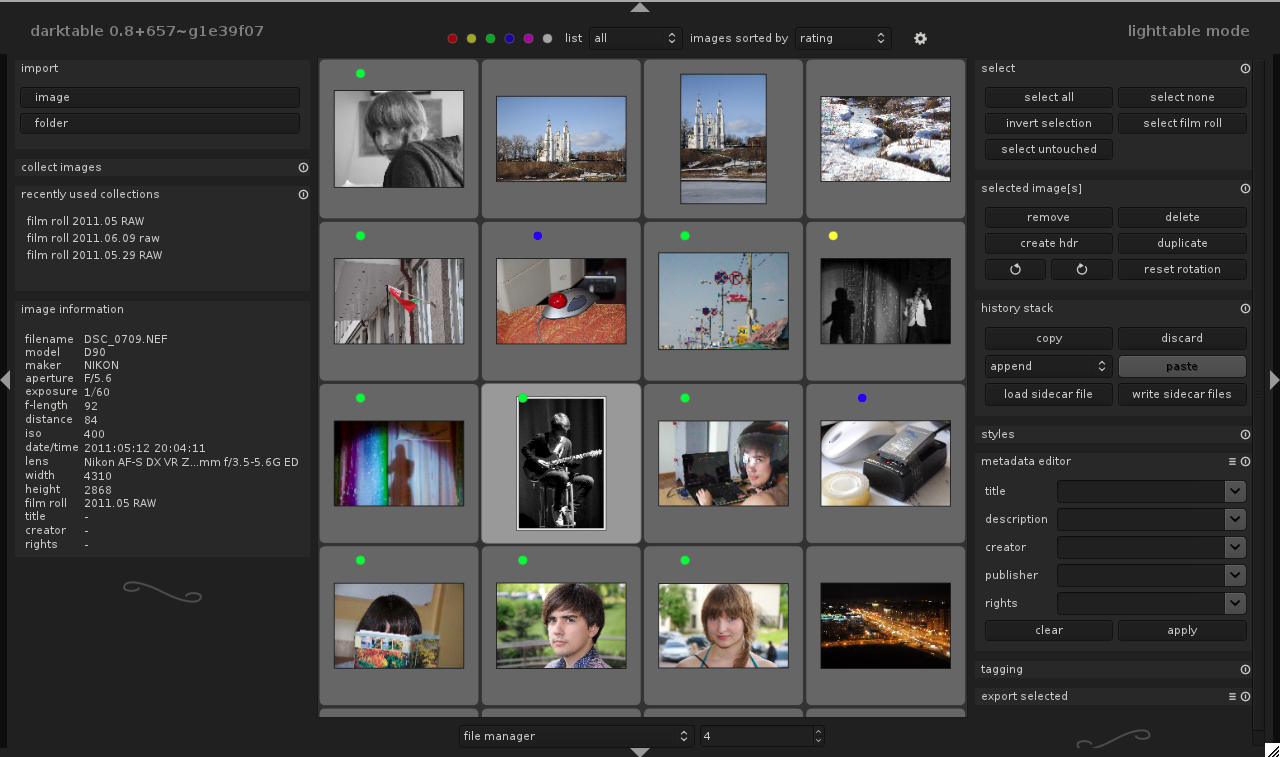
\includegraphics[width=11cm]{11_darktable_01.png}}
%\label{pic:fl1}
%\caption{Приложения по категориям}
\end{figure}
\begin{figure}[ht]
\centering{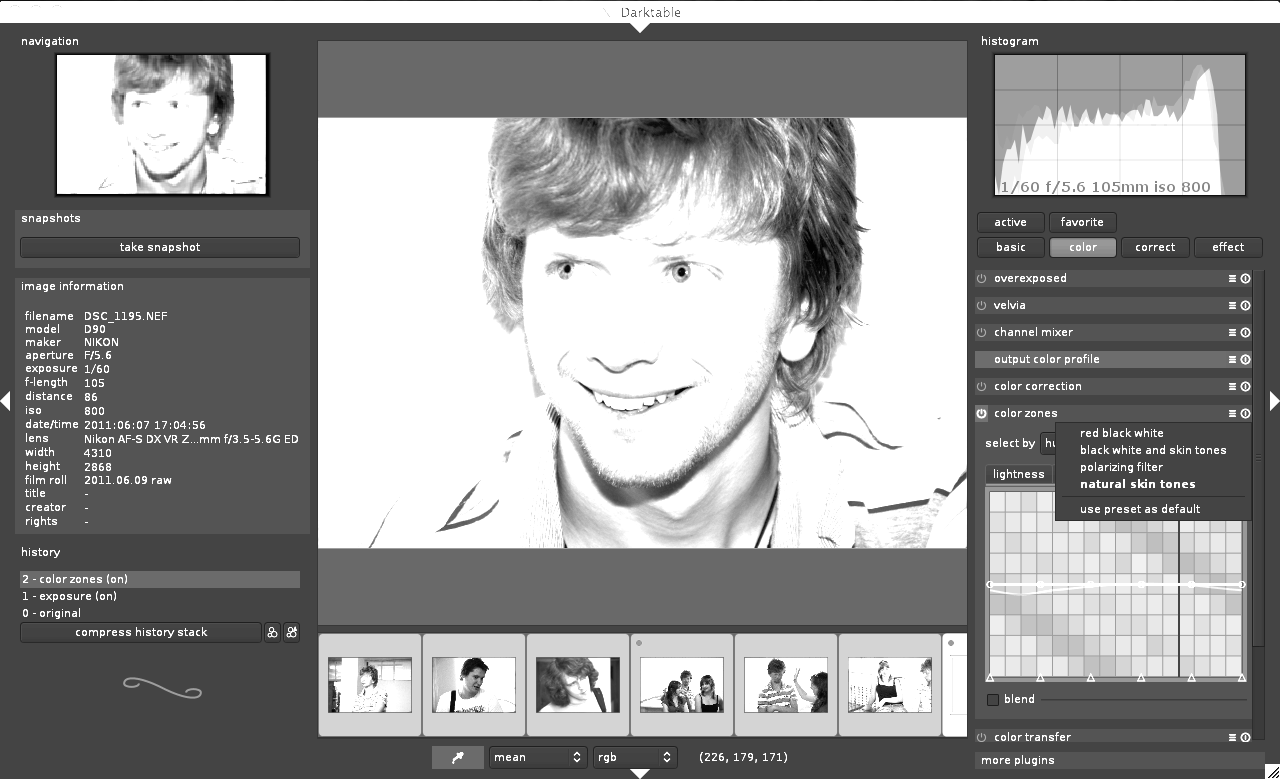
\includegraphics[width=11cm]{11_darktable_02.png}}
%\label{pic:fl1}
%\caption{Приложения по категориям}
\end{figure}

Логически модули можно разделить на следующие категории: основная, цвет, корреция и эффекты.
К модулям работы с цветом относятся:
\begin{itemize}
\item вельвия
\item регулирование яркости/насыщенности или сдвига тонов в плагине цветовые зоны
\item микшер каналов
\item алгоритмы дебайеризации ppg и AMaZE 
\item поканальный баланс белого через множители либо через  - сдвиг цветовой температуры и множителя зеленого канала
\item редактируемая тональная кривая камеры с возможностью выбора из набора готовых кривых, аналогичных используемым производителями цифровых фотоаппаратов
\item восстановление пересветов при отрицательной экспокоррекции
\item профили камеры: стандартные (Adobe), улучшенные, либо пользовательские
\end{itemize}
Модули коррекции изображения включают:
\begin{itemize}
\item трансформации: кадрирование с выбираемым соотношением сторон, поворот, перспектива
\item исправление геометрических искажений оптики с помощью библиотеки lensfun
\item редактируемая тональная кривая (L канал в LCh пространстве
\item возможность работать с тональной кривой в виде последовательности зон Адамса
\item мощнейший инструмент --- эквалайзер, позволяющий регулировать локальный контраст (L и С) в зависимости от пространственной частоты (аналога радиуса в USM) с помощью избегающих краев вейвлетов
\item подавление шума
\end{itemize}
И, наконец, основные модули эффектов:
\begin{itemize}
\item обесцвечивание с регулируемым цветовым фильтром
\item градиентный фильтр (GND) с возможностью поворота и радиального смещения
\item эффект виньетирования с регулируемыми на холсте радиусом, формой (окружность/эллипс)
\item смягчающий фильтр
\end{itemize}

\section*{Будущее}
В настоящее время разработчики готовят программу к выпуску версии 0.9. 

В ближайших планах разработчиков --- добавление функционала масок (Henrik Andersson) и переработка интерфейса с централизованной обработкой горячих клавиш (GSoC студент Robert Bieber). В состоянии обсуждения — возможность не  однократного использования плагинов. В более отдаленных планах — использование GEGL внутри darktable с возможностью передачи данных в GIMP и обратно для более сложного редактирования; однако этот функционал может появиться не раньше выхода GIMP 3.0.

Проект активно развивается и радует постоянное растущее сообщество пользователей новыми выпусками с периодичностью примерно раз в три месяца. Можно ответственно заявить, что текущая версия пригодна для использования профессиональным фотографом.

\begin{thebibliography}{9}
\bibitem{pDynamo} Официальный сайт проекта --- \url{http://darktable.sf.net}
\end{thebibliography}
\end{document}
